\documentclass[aps,pra,twocolumn,reprint,floatfix,amsmath,amssymb]{revtex4-2}

\usepackage{graphicx}
\usepackage{booktabs}
\usepackage{siunitx}
\usepackage[colorlinks=true,linkcolor=blue,citecolor=blue,urlcolor=blue]{hyperref}
\usepackage{float}
\usepackage{xcolor}

\begin{document}

\title{Can Parameterized Waveforms Realize an Ideal SQR Gate? Direct and Echoed Multitone Tests}
\author{Codex}
\affiliation{cQED Autonomous Research Platform}
\date{\today}

\begin{abstract}
We revisit two earlier repository studies that approached selective qubit rotation (SQR) control with multitone Gaussian pulses, but did not directly answer whether a parameterized waveform can realize an ideal SQR gate. The first earlier study optimized arbitrary block-diagonal SU(2) targets, which is broader than an ideal SQR. The second used a different echoed construction and a scalarized residual-$Z$ objective rather than the requested ideal-SQR target. In this follow-up we target the narrower unitary $U_{\mathrm{SQR}}^{\mathrm{ideal}}=\sum_n |n\rangle\langle n|\otimes R_x(\theta_n)$ and compare four constructions on a 16-case grid: a direct multitone waveform, a fully symmetric echoed waveform built from two half-SQR segments and two finite $X_\pi$ pulses, an equal-duration echoed waveform with independent half-segment corrections, and a weakly asymmetric echoed waveform with small duration imbalance. A low-dimensional analytic treatment predicts that a symmetric echo can cancel first-order residual $Z$ phase only if the inserted refocusing pulses are effectively manifold independent. The numerical study, performed with \texttt{cqed\_sim} plus a small local wrapper for composite-sequence optimization, shows the opposite practical trend: the direct construction outperforms all echoed variants in every tested case. Its mean average gate fidelity is $0.595$, compared with $0.248$ for the echoed families, and its mean residual-$Z$ error is also smaller. Allowing independent echoed corrections changes only the fifth decimal place, while the asymmetric optimization never selects nonzero timing asymmetry. Within this parameterization family, no candidate realizes a near-ideal SQR gate, and the most credible path remains the direct multitone baseline rather than the echoed constructions.
\end{abstract}

\maketitle

\section{Introduction}
Selective qubit rotations conditioned on cavity Fock number are a natural control primitive in dispersive circuit quantum electrodynamics (cQED) \cite{blais2021cqed,koch2007transmon}. In the idealized picture one chooses rotation angles $\theta_n$ and implements
\begin{equation}
U_{\mathrm{SQR}}^{\mathrm{ideal}}(\{\theta_n\})=
\sum_{n=0}^{N_{\mathrm{active}}-1}|n\rangle\langle n|\otimes R_x(\theta_n),
\qquad
R_x(\theta)=e^{-i\theta \sigma_x/2},
\end{equation}
with a common qubit rotation axis and no residual block-dependent phase.

Two earlier repository studies came close to this question without actually resolving it. The study \texttt{multitone\_sqr\_arbitrary\_fock\_conditional\_rotations} optimized arbitrary blockwise SU(2) targets, not an ideal SQR gate. The study \texttt{parameterized\_waveform\_residual\_z\_cancellation} introduced richer parameterizations, but its ``echoed'' pulse family used a different composite schedule and a scalarized fidelity-plus-residual-$Z$ loss rather than the pure ideal-SQR target requested here. Those differences matter because the algebra of an echoed cancellation scheme is only clean when the target axis is fixed.

This follow-up therefore asks a narrower and sharper question: does there exist a multitone waveform parameterization, direct or echoed, that can realize an ideal SQR gate in a physically credible way? We compare a direct multitone Gaussian-envelope waveform against an echoed sequence of the form
\begin{equation}
\text{half-SQR}\rightarrow X_\pi\rightarrow \text{half-SQR}\rightarrow X_\pi,
\end{equation}
and study three echoed variants: fully symmetric, equal-duration with independent half corrections, and weakly asymmetric with small duration imbalance. Before numerics, we derive the low-$n$ first-order conditions needed for direct and echoed success. The remainder of the paper introduces the model and parameterizations, reports the critical audit of the earlier studies, compares numerical outcomes, validates the results, and closes with a direct answer to whether any of these constructions offers a convincing path to an ideal or near-ideal SQR gate.

\section{System and Methods}

\subsection{Hamiltonian}
All simulations use the dispersive transmon-cavity model implemented in \texttt{cqed\_sim} \cite{cqedsim2026}. Because the working transmon truncation is $n_{\mathrm{tr}}=2$, the qubit Hilbert space is effectively two level and the excitation projector is $n_q=|e\rangle\langle e|$. The Hamiltonian in the lab frame is
\begin{equation}
\frac{H_0}{\hbar}
=
\omega_c a^\dagger a
+ \omega_q n_q
+ \chi\, a^\dagger a\, n_q
+ \chi' a^\dagger a (a^\dagger a-1) n_q,
\label{eq:hamiltonian}
\end{equation}
with the $\chi'$ term present only in the \texttt{chi\_plus\_chiprime} model variant. The code retains the transmon anharmonicity parameter $\alpha$, but because $n_{\mathrm{tr}}=2$ there is no populated second excited state and $\alpha$ does not affect the simulated dynamics in this study. Drives act on the qubit channel only.

\subsection{Simulation Parameters}
Table~\ref{tab:params} lists the fixed model and pulse parameters. The main study grid spans two model variants, two target families, two active-window sizes, and two total SQR durations, giving 16 cases and 64 saved construction rows.

\begin{table*}[t]
\centering
\caption{System and numerical parameters used in the follow-up study. The cavity truncation is $N_{\mathrm{cav}}=N_{\mathrm{active}}+2$ in the main runs and is increased to $N_{\mathrm{active}}+3$ in the convergence check.}
\label{tab:params}
\begin{tabular}{@{}lll@{}}
\toprule
Parameter & Value & Notes \\
\midrule
$\omega_q/2\pi$ & \SI{6.150}{\giga\hertz} & Bare qubit frequency \\
$\omega_c/2\pi$ & \SI{5.241}{\giga\hertz} & Bare cavity frequency \\
$\alpha/2\pi$ & \SI{-255}{\mega\hertz} & Present in model definition, inactive for $n_{\mathrm{tr}}=2$ \\
$\chi/2\pi$ & \SI{-2.84}{\mega\hertz} & Dispersive shift \\
$\chi'/2\pi$ & \SI{-21}{\kilo\hertz} & Enabled only in \texttt{chi\_plus\_chiprime} \\
$n_{\mathrm{tr}}$ & $2$ & Two-level qubit truncation \\
$N_{\mathrm{active}}$ & $2,3$ & Active Fock blocks targeted in the main grid \\
$N_{\mathrm{cav}}$ & $N_{\mathrm{active}}+2$ & Main truncation \\
$|\chi|T/2\pi$ & $3,5$ & Active SQR duration grid \\
$dt$ & \SI{4}{\nano\second} & Main compiler step; \SI{2}{\nano\second} for convergence check \\
Gaussian envelope width & $\sigma=T/6$ & Shared by direct and half-SQR multitone segments \\
$X_\pi$ duration & \SI{40}{\nano\second} & Finite Gaussian refocusing pulse \\
$X_\pi$ width & $\sigma=T_\pi/4$ & Refocusing pulse envelope width \\
Direct optimizer weights & $(0.15,1.0,0.35,0.35)$ & Qubit, subspace, preservation, leakage weights \\
Direct correction bounds & $\delta\lambda\in[-0.75,0.75]$, $\delta\alpha\in[-\pi,\pi]$, $\delta\omega/2\pi\in[-3,3]$ MHz & Public \texttt{cqed\_sim} optimizer \\
Echo asymmetry bound & $\eta\in[-0.15,0.15]$ & Only in the weakly asymmetric case \\
\bottomrule
\end{tabular}
\end{table*}

The ideal target angles are chosen deterministically to probe two qualitatively different gate families:
\begin{align}
\texttt{smooth\_x}: \quad
\theta_n &= \min\!\bigl(0.30\pi + 0.18\pi n,\, 0.92\pi\bigr),\\
\texttt{staggered\_x}: \quad
\theta_n &= \min\!\bigl(0.22\pi + 0.58\pi (n\bmod 2) + 0.06\pi \lfloor n/2 \rfloor,\, 0.94\pi\bigr).
\end{align}
The first family is a smooth monotone profile; the second is intentionally harder because adjacent manifolds demand more uneven rotations.

\subsection{Analytic Preliminary}
The direct multitone waveform can be viewed, within each active Fock manifold $n$, as an effective driven qubit with desired $x$ rotation area $\Theta_n$ and undesired residual $Z$ phase $\Phi_n$. To first order,
\begin{equation}
U_n^{\mathrm{dir}}
\approx
\exp\!\left[-\frac{i}{2}\bigl(\Theta_n X + \Phi_n Z\bigr)\right].
\label{eq:direct_first_order}
\end{equation}
An ideal direct SQR therefore requires
\begin{equation}
\Theta_n=\theta_n,\qquad \Phi_n=0
\qquad \text{for every active manifold } n.
\end{equation}

For the echoed construction we write the two half segments as
\begin{equation}
U_{n,j}^{\mathrm{half}}
\approx
\exp\!\left[-\frac{i}{2}\bigl(\Theta_{n,j} X + \Phi_{n,j} Z\bigr)\right],
\qquad j\in\{1,2\},
\end{equation}
and insert ideal $X_\pi=-iX$ pulses. Using $X_\pi X X_\pi = X$ and $X_\pi Z X_\pi = -Z$, the echoed block reduces at first order to
\begin{equation}
U_n^{\mathrm{echo}}
\approx
\exp\!\left[-\frac{i}{2}\bigl((\Theta_{n,1}+\Theta_{n,2})X + (\Phi_{n,1}-\Phi_{n,2})Z\bigr)\right].
\label{eq:echo_first_order}
\end{equation}
This produces three immediate low-$n$ conclusions.

First, for $N_{\mathrm{active}}=1$ the symmetric echo should be nearly equivalent to the direct waveform because both halves see the same single manifold and first-order residual $Z$ cancels automatically if $\Phi_{0,1}=\Phi_{0,2}$. Second, for $N_{\mathrm{active}}=2$ or $3$, a fully symmetric echoed construction can still cancel first-order residual $Z$ manifold by manifold, but only if the inserted refocusing pulses act uniformly across the active manifolds. Third, the mechanism is fragile: finite refocusing pulses generate their own manifold-dependent coherent errors, and second-order commutators reintroduce transverse error terms. The echoed idea is therefore plausible in principle, but only in the ideal toggling-frame limit.

\subsection{Computational Approach}
The direct multitone ansatz used throughout the study is
\begin{equation}
\Omega_{\mathrm{dir}}(t)
=
g_T(t)\sum_{n=0}^{N_{\mathrm{active}}-1}
\lambda_n^{(0)}\bigl(1+\delta\lambda_n\bigr)
e^{i[(\omega_n^{(0)}+\delta\omega_n)t+\delta\alpha_n]},
\label{eq:direct_ansatz}
\end{equation}
where $g_T(t)$ is the Gaussian envelope used by \texttt{cqed\_sim}, centered at $T/2$ with width $\sigma=T/6$, and $\lambda_n^{(0)}$, $\omega_n^{(0)}$ are the nominal per-manifold tone amplitudes and transition frequencies generated from the ideal target. The optimized correction parameters are therefore $\{\delta\lambda_n,\delta\alpha_n,\delta\omega_n\}$.

The echoed construction uses the same ansatz for each half segment but with half-angle targets $\theta_n/2$. The three echoed variants are
\begin{align}
\text{Symmetric:} \quad & \mathbf{c}_1=\mathbf{c}_2,\; T_1=T_2=T/2, \\
\text{Independent:} \quad & \mathbf{c}_1\neq \mathbf{c}_2,\; T_1=T_2=T/2, \\
\text{Asymmetric:} \quad & \mathbf{c}_1\neq \mathbf{c}_2,\; T_1=\tfrac{T}{2}(1+\eta),\; T_2=\tfrac{T}{2}(1-\eta),
\end{align}
with $\mathbf{c}_j=(\delta\lambda^{(j)},\delta\alpha^{(j)},\delta\omega^{(j)})$ and $|\eta|\le 0.15$.

The direct waveform and the symmetric half-SQR seed are optimized entirely within the public \texttt{cqed\_sim} API using \texttt{optimize\_targeted\_subspace\_multitone}. The target operator is always the ideal SQR unitary of Eq.~(1), and the direct loss is the framework weighted objective
\begin{equation}
\mathcal{L}_{\mathrm{dir}}
=
0.15\,L_{\mathrm{qubit}}
+1.00\,L_{\mathrm{subspace}}
+0.35\,L_{\mathrm{preservation}}
+0.35\,L_{\mathrm{leakage}}.
\end{equation}

The equal-duration and asymmetric echoed cases expose a public-API gap: \texttt{cqed\_sim} does not yet provide a multi-segment targeted-subspace optimizer. We therefore built only the outer composite wrapper locally while keeping the model, pulse generation, compilation, and simulation inside \texttt{cqed\_sim}. The echoed local objective is
\begin{equation}
\mathcal{L}_{\mathrm{echo}}
=
\mathcal{L}_{\mathrm{dir-like}}
+0.05\,\overline{\epsilon_Z}
+10^{-5}\|\mathbf{x}-\mathbf{x}_{\mathrm{seed}}\|^2
+0.01|\eta|,
\label{eq:echo_objective}
\end{equation}
where $\overline{\epsilon_Z}$ is the mean residual-$Z$ block error and $\eta=0$ in the equal-duration case. We used Powell optimization with up to 70 function evaluations for equal-duration independent corrections and 80 for the asymmetric case.

\section{Results}

\subsection{Critical Audit of the Earlier Studies}
The first outcome of the follow-up is negative but important: neither earlier study had actually answered the present question. The arbitrary-rotation study solved a broader control problem, so its success or failure could not be interpreted as success or failure of an ideal SQR gate. The residual-$Z$ study, despite being closer in spirit, did not implement the requested
\begin{equation}
\text{half-SQR}\rightarrow X_\pi\rightarrow \text{half-SQR}\rightarrow X_\pi
\end{equation}
schedule, and its objective was not the ideal-SQR unitary itself. Both earlier studies were therefore informative baselines, but neither one was a definitive test of whether an ideal SQR gate exists inside the narrower direct or echoed parameterizations studied here.

\subsection{Direct Versus Echoed Constructions}
Figure~\ref{fig:construction_means} shows the clearest numerical message: the direct multitone waveform outperforms every echoed construction on mean average gate fidelity, and it also has the smallest mean residual-$Z$ error. Across the full 16-case grid the direct construction achieves a mean average fidelity of $0.5951$, while the echoed families cluster tightly near $0.2482$. The mean residual-$Z$ error is $0.0582$ rad for the direct waveform and about $0.318$ rad for all echoed families.

\begin{figure}[t]
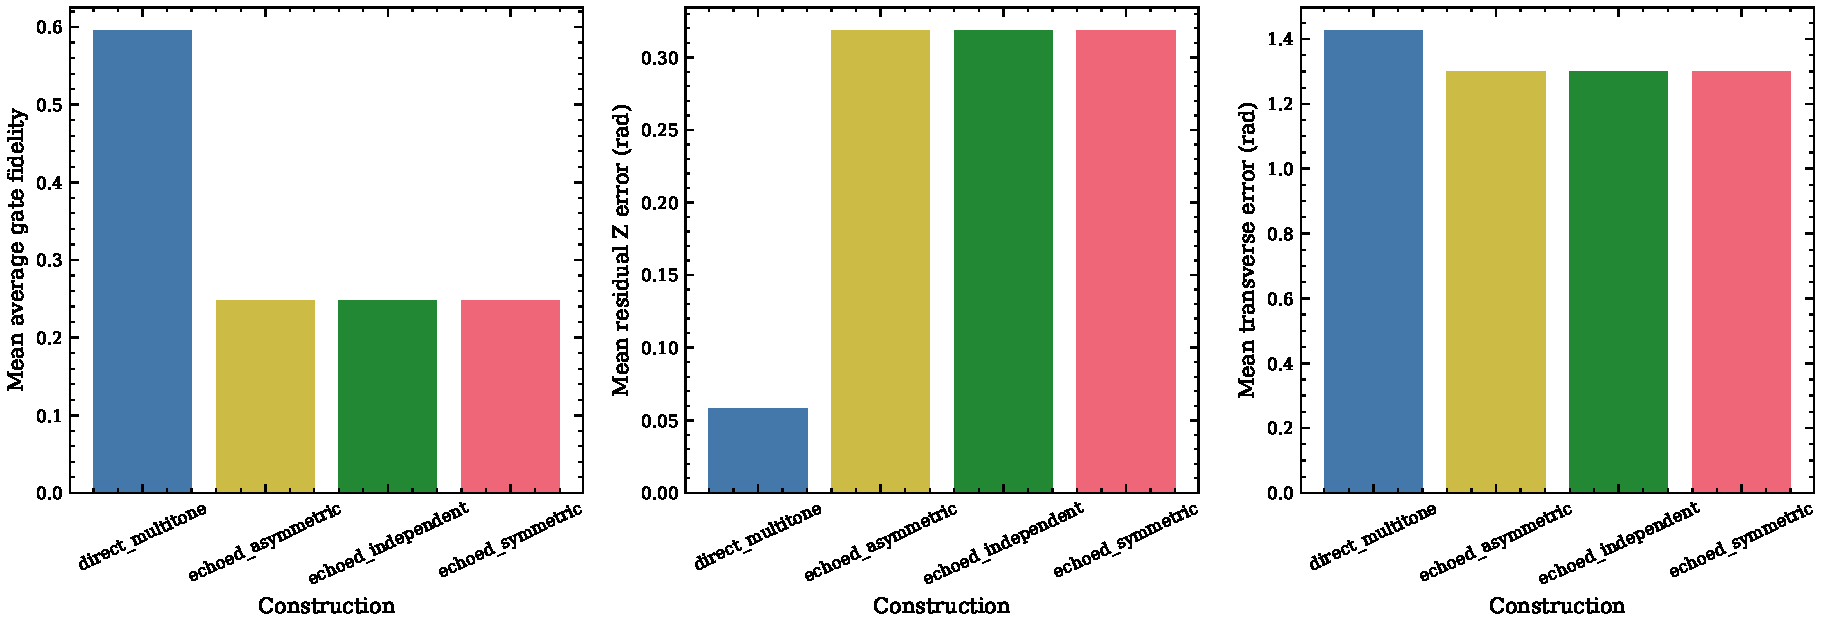
\includegraphics[width=\columnwidth]{../figures/construction_metric_means.pdf}
\caption{Mean performance metrics across all 16 study cases. The direct multitone waveform has the highest mean fidelity and the smallest mean residual-$Z$ error. The echoed families have slightly smaller mean transverse error, but not enough to compensate for the large fidelity loss and residual-$Z$ penalty.}
\label{fig:construction_means}
\end{figure}

The duration-resolved comparison in Fig.~\ref{fig:duration_tradeoff} shows that increasing $|\chi|T/2\pi$ from $3$ to $5$ helps the direct waveform modestly, especially for the smoother target family, but does not rescue any echoed construction. The case-by-case heatmap in Fig.~\ref{fig:heatmap} makes the stronger statement: the direct waveform wins in all 16 matched cases.

\begin{figure}[t]
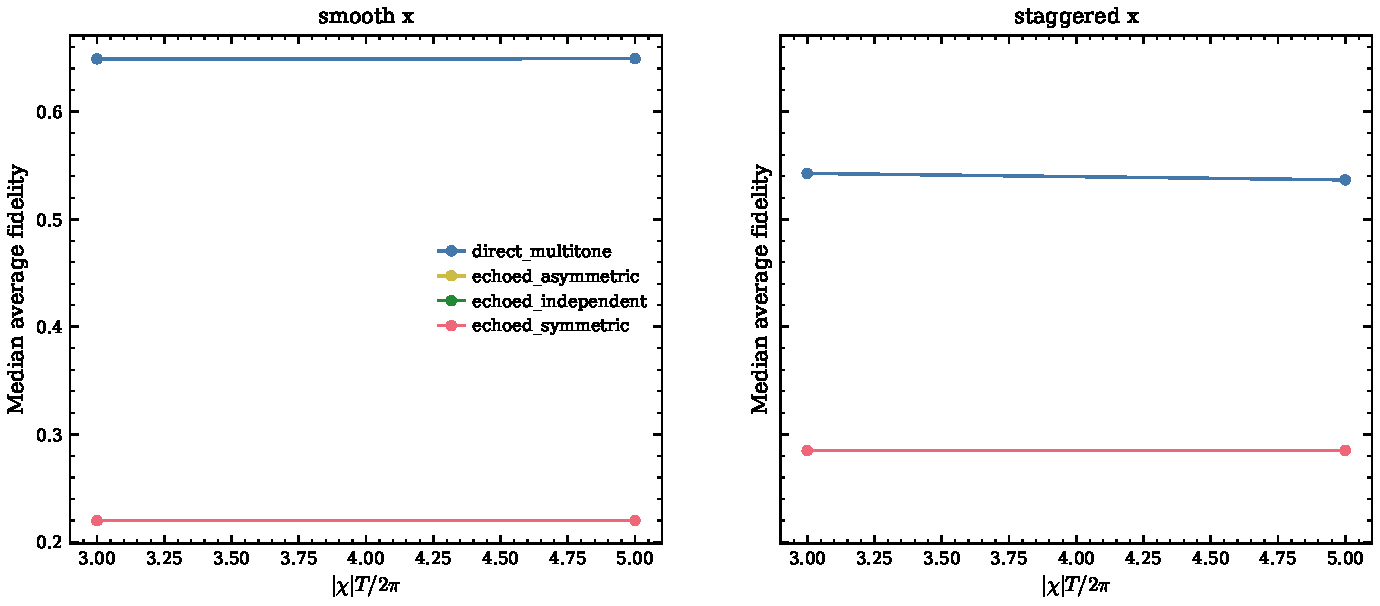
\includegraphics[width=\columnwidth]{../figures/duration_fidelity_tradeoff.pdf}
\caption{Median average fidelity versus normalized active SQR duration for the two target families. The direct waveform benefits modestly from the longer duration, whereas the echoed constructions remain far below it for both target families.}
\label{fig:duration_tradeoff}
\end{figure}

\begin{figure}[t]
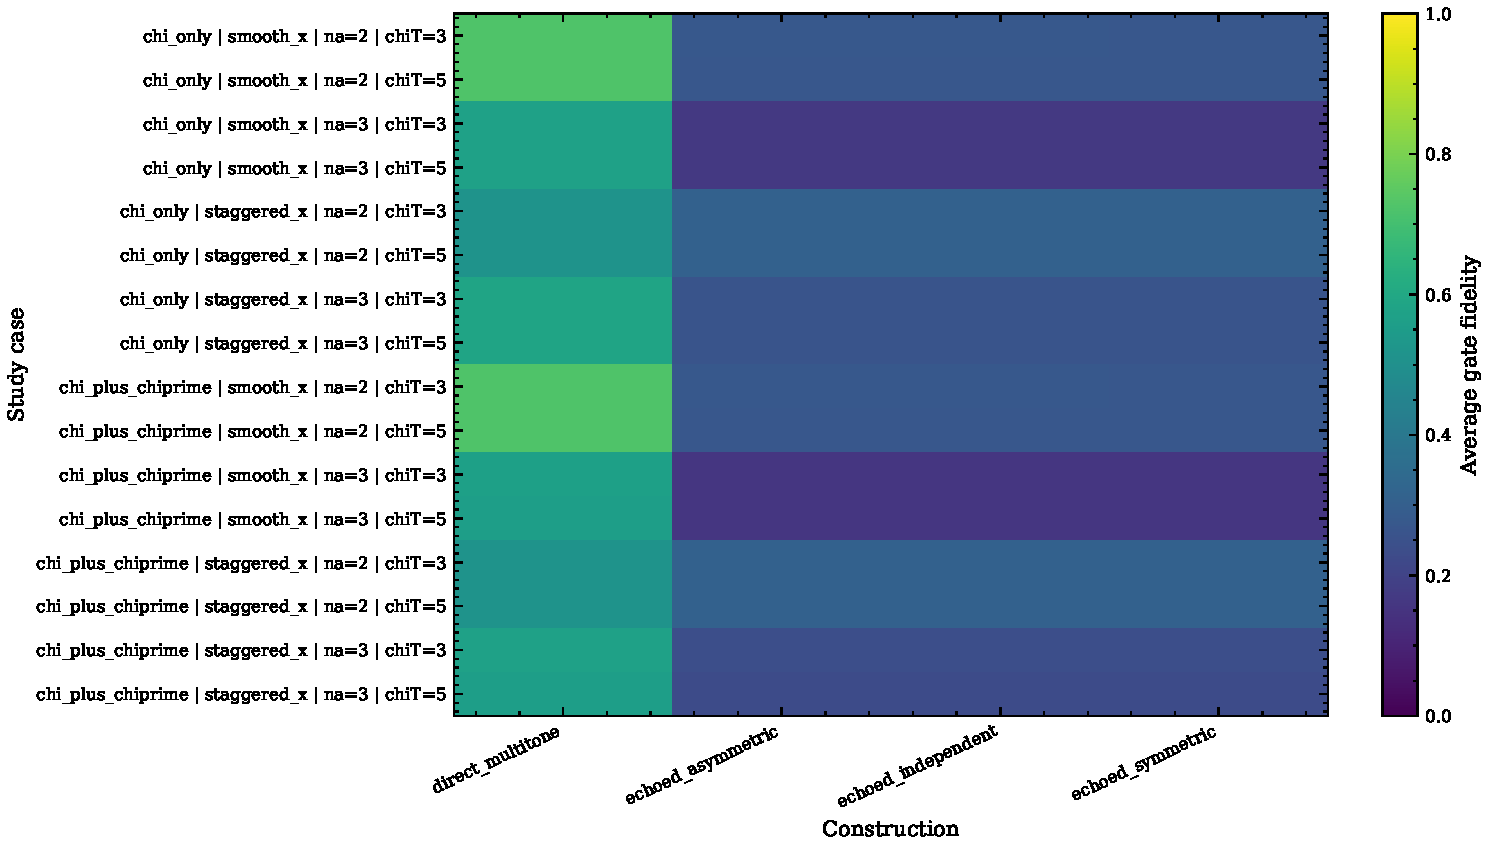
\includegraphics[width=\columnwidth]{../figures/case_construction_heatmap.pdf}
\caption{Average gate fidelity for every saved case and construction. Each row is one of the 16 study cases. The direct multitone construction is the best performer in every row.}
\label{fig:heatmap}
\end{figure}

The best overall case is the direct waveform for the \texttt{chi\_only}, \texttt{smooth\_x}, $N_{\mathrm{active}}=2$, $|\chi|T/2\pi=5$ setting, with average gate fidelity $0.72454$. This is the most successful parameterization found in the study, but it is still far from a near-ideal gate. Its per-block residual-$Z$ errors are only $0.00168$ and $0.05069$ rad, while the larger coherent failure comes from transverse and angle mismatch. In other words, even the best direct solution is not mainly limited by leftover $Z$ phase.

\subsection{Does Echo Cancel Residual $Z$, Reduce It, or Redistribute Error?}
Figure~\ref{fig:delta_tradeoff} compares each echoed row to the matched direct row. No echoed construction produces a net fidelity gain. The mean change relative to direct is
\begin{align}
\langle \Delta F_{\mathrm{avg}}\rangle &\approx -0.3469,\\
\langle \Delta \overline{\epsilon_Z}\rangle &\approx +0.2601~\mathrm{rad},\\
\langle \Delta \overline{\epsilon_\perp}\rangle &\approx -0.1249~\mathrm{rad},
\end{align}
where $\overline{\epsilon_\perp}$ denotes the mean transverse coherent error extracted from the per-block error generator.

\begin{figure}[t]
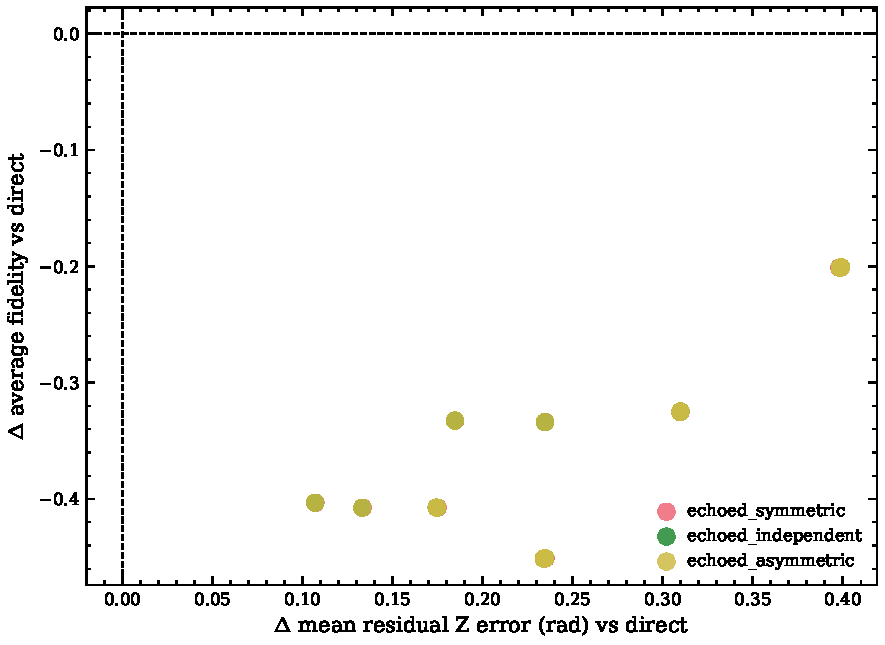
\includegraphics[width=\columnwidth]{../figures/echo_delta_tradeoff.pdf}
\caption{Change in mean residual-$Z$ error and average fidelity for each echoed construction relative to the matched direct waveform. All points lie below the zero-fidelity line. Echoed sequences sometimes reduce transverse error, but not residual-$Z$, and never enough to outperform the direct construction.}
\label{fig:delta_tradeoff}
\end{figure}

This is the opposite of the hoped-for narrative. The echoed constructions do not cancel residual-$Z$ error in practice. At best they redistribute coherent error: transverse components are slightly smaller on average, but residual-$Z$ becomes much larger and the net gate quality worsens.

\subsection{Symmetry, Independent Corrections, and Asymmetry}
The three echoed cases are nearly indistinguishable numerically. The fully symmetric echo has mean average fidelity $0.248211$. Allowing independent half-segment correction parameters increases this only to $0.248217$. The asymmetric case reaches $0.248217$ as well, and every best-fit asymmetric artifact returns $\eta=0$ within numerical tolerance. That behavior answers two of the main design questions directly.

First, independent half corrections do not materially improve the echoed protocol. They change the fifth decimal place, not the physical conclusion. Second, the extra duration degree of freedom provides no meaningful advantage at all inside this parameterization family. The optimizer never prefers a nonzero timing asymmetry, so there is no evidence that weak asymmetry unlocks a hidden high-fidelity echo solution.

\section{Validation}
All three required validation checks were completed.

\subsection{Sanity Checks}
The cleanest sanity check is the single-manifold limit $N_{\mathrm{active}}=1$ for the \texttt{chi\_only}, \texttt{smooth\_x}, $|\chi|T/2\pi=5$ case. Here the first-order analytic argument predicts that the symmetric echo should behave almost like the direct construction. The measured average fidelities are $0.862605$ for the direct waveform and $0.862477$ for the symmetric echo, a difference of only $1.28\times 10^{-4}$. This confirms that the numerical machinery reproduces the expected low-dimensional limit.

\subsection{Convergence Analysis}
We repeated the best direct and best echoed cases with a smaller time step $dt=\SI{2}{\nano\second}$ and with one additional cavity Fock level. The best direct case shifts from $0.7245389644$ to $0.7248270938$ under the finer time step and to $0.7245387313$ under the larger cavity truncation. The best echoed case shifts from $0.3113412141$ to $0.3109023176$ and to $0.3113410880$ under the same checks. All changes are below $5\times 10^{-4}$ in fidelity, so the numerical ranking is stable.

\subsection{Literature Comparison}
There is no direct literature benchmark for the exact question posed here because the main purpose of this follow-up is to adjudicate between local repository constructions rather than reproduce a published gate benchmark. We therefore report the literature comparison as not applicable for this focused study.

\section{Discussion}
The key analytic and numerical conclusions fit together cleanly. The low-$n$ algebra says that a symmetric echo could cancel first-order residual-$Z$ phase if the two halves are identical and the refocusing pulses are effectively manifold independent. The numerical simulations show that this ideal toggling-frame picture is not realized by the actual finite Gaussian $X_\pi$ pulses. Once the refocusing pulses themselves are manifold dependent, the symmetry argument weakens enough that the echoed construction becomes worse, not better.

This also clarifies why the direct waveform remains the best available option in the present family despite being far from ideal. Its dominant failures are not purely residual-$Z$ effects; even the best direct result already has small residual-$Z$ but substantial axis and angle mismatch. The echoed construction does not address that broader coherent-control limitation and introduces additional refocusing-pulse structure that worsens the net result. The weakly asymmetric case is especially revealing: if echoed improvement required a delicate timing skew, one might have argued that the clean symmetric idea was incomplete but salvageable. Instead, the optimizer repeatedly returns $\eta=0$, so there is no sign of a hidden asymmetric mechanism waiting to be exploited.

From a physical plausibility standpoint, the direct multitone waveform is therefore the more convincing baseline. It is simpler, shorter in total duration, and consistently better than all echoed variants. Nevertheless, no construction studied here reaches a near-ideal SQR gate. Under this ansatz family the evidence points toward a real obstruction, not merely insufficient tuning.

\section{Conclusion}
This follow-up study gives a direct answer to the central question. A direct multitone Gaussian-envelope waveform is the strongest candidate among the tested parameterizations, but it does not realize an ideal or near-ideal SQR gate on the present grid; the best average fidelity is only $0.72454$. A fully symmetric echoed multitone waveform does not do better. Allowing independent half-segment corrections changes the result only marginally, and allowing weak timing asymmetry produces no practical gain at all because the optimizer returns $\eta=0$ in every best-fit saved artifact.

The six motivating questions can therefore be answered succinctly. The direct waveform can realize a moderate-quality but not near-ideal SQR gate. The fully symmetric echo does not improve upon it and does not cancel residual-$Z$ effects in practice. Independent half corrections do not materially help. Meaningful improvement does not appear only after timing asymmetry, because no timing asymmetry is actually selected. Consequently there is no evidence that the echoed construction is a more fundamental or more robust route to an ideal SQR gate. Finally, the small-$n$ analytics say the ideal echo cancellation is achievable only in principle, in the limit of effectively manifold-independent refocusing pulses; the finite-pulse simulations show that this idealization is not realized here.

\section{Limitations and Future Work}

\subsection{Known Limitations}
The main technical limitation is that \texttt{cqed\_sim} currently exposes a public optimizer for single-segment targeted-subspace multitone waveforms but not for multi-segment composite sequences. The direct waveform therefore stays entirely inside the public API, while the equal-duration and asymmetric echoed cases require a thin local optimization wrapper. This does not affect the simulated physics, but it does mean the echoed optimization landscape was explored with a smaller bespoke loop.

The second limitation is conceptual: the echoed verdict depends on the finite Gaussian $X_\pi$ pulses used to realize the refocusing step. Because those pulses are themselves manifold dependent, the present study cannot separate ``echo failure as a matter of principle'' from ``echo failure because the available refocusing pulses are not ideal enough.'' That distinction matters for future work, even though it does not change the present numerical conclusion.

The third limitation is scope. We focused on ideal $x$-axis SQR gates with $N_{\mathrm{active}}=2,3$ in order to keep the low-dimensional analytic story interpretable and the numerical grid tractable. A broader target family or larger active window could reveal additional behavior, although the present trends are already strong.

\subsection{Suggested Improvements}
\begin{itemize}
  \item \textbf{[P1 | MEDIUM]} Add a public \texttt{cqed\_sim} optimizer for composite targeted-subspace sequences so that direct and echoed ansatz families can be compared on equal footing inside the same optimization framework.
  \item \textbf{[P1 | MEDIUM]} Upgrade the echoed construction to use manifold-robust or jointly optimized refocusing pulses. This is the clearest way to test whether the present echoed failure is caused mainly by the finite $X_\pi$ pulses rather than by the multitone halves.
  \item \textbf{[P2 | MEDIUM]} Extend the target family beyond fixed $x$-axis rotations to check whether a different common axis or a broader ideal-SQR convention is easier to realize while remaining physically meaningful.
  \item \textbf{[P2 | LOW]} Push the active-window grid to $N_{\mathrm{active}}=4$ once the composite optimizer is improved, to test whether the direct-over-echoed ranking persists under stronger spectral crowding.
  \item \textbf{[P3 | LOW]} Export a machine-readable analytic summary table linking each numerical case to its direct and echoed first-order expectations, to make future cross-study comparisons easier.
\end{itemize}

\subsection{Open Questions}
The main open question is whether an echoed SQR could become competitive once the refocusing pulses themselves are upgraded. A second unresolved issue is whether the direct ansatz fails because it lacks enough independent frequency-domain structure, or because the ideal SQR target is genuinely incompatible with simple Gaussian multitone control on the explored manifolds. A third question is whether a broader control family can reduce the large transverse coherent errors seen even in the best direct solution without reintroducing substantial residual-$Z$ phase.

\bibliographystyle{apsrev4-2}
\bibliography{references}

\appendix

\section{Detailed Results and Data}
Table~\ref{tab:construction_summary} summarizes the mean construction-level metrics. The direct waveform is best by every fidelity-based measure. Table~\ref{tab:best_cases} lists the best saved case for each construction family.

\begin{table*}[h]
\centering
\caption{Construction-level averages across the 16-case grid.}
\label{tab:construction_summary}
\begin{tabular}{@{}lcccc@{}}
\toprule
Construction & Mean average fidelity & Best average fidelity & Mean residual-$Z$ (rad) & Mean transverse error (rad) \\
\midrule
Direct multitone & 0.595142 & 0.724539 & 0.058152 & 1.425383 \\
Echoed asymmetric & 0.248217 & 0.311341 & 0.318238 & 1.300471 \\
Echoed independent & 0.248217 & 0.311341 & 0.318240 & 1.300469 \\
Echoed symmetric & 0.248211 & 0.311322 & 0.318233 & 1.300564 \\
\bottomrule
\end{tabular}
\end{table*}

\begin{table*}[h]
\centering
\caption{Best saved case for each construction. The asymmetric echoed winner still has $\eta=0$, so its best point is effectively equal-duration.}
\label{tab:best_cases}
\begin{tabular}{@{}llllcc@{}}
\toprule
Construction & Case ID & Target family & Model & Average fidelity & Mean residual-$Z$ (rad) \\
\midrule
Direct multitone & \texttt{chi\_only\_smooth\_x\_na2\_chiT5p0} & \texttt{smooth\_x} & \texttt{chi\_only} & 0.724539 & 0.026186 \\
Echoed symmetric & \texttt{chi\_plus\_chiprime\_staggered\_x\_na2\_chiT3p0} & \texttt{staggered\_x} & \texttt{chi\_plus\_chiprime} & 0.311322 & 0.414455 \\
Echoed independent & \texttt{chi\_plus\_chiprime\_staggered\_x\_na2\_chiT3p0} & \texttt{staggered\_x} & \texttt{chi\_plus\_chiprime} & 0.311341 & 0.414932 \\
Echoed asymmetric & \texttt{chi\_plus\_chiprime\_staggered\_x\_na2\_chiT3p0} & \texttt{staggered\_x} & \texttt{chi\_plus\_chiprime} & 0.311341 & 0.414932 \\
\bottomrule
\end{tabular}
\end{table*}

Figure~\ref{fig:appendix_waveforms} shows representative direct and echoed baseband waveforms for a difficult \texttt{chi\_plus\_chiprime}, \texttt{staggered\_x}, $N_{\mathrm{active}}=3$, $|\chi|T/2\pi=5$ case.

\begin{figure*}[h]
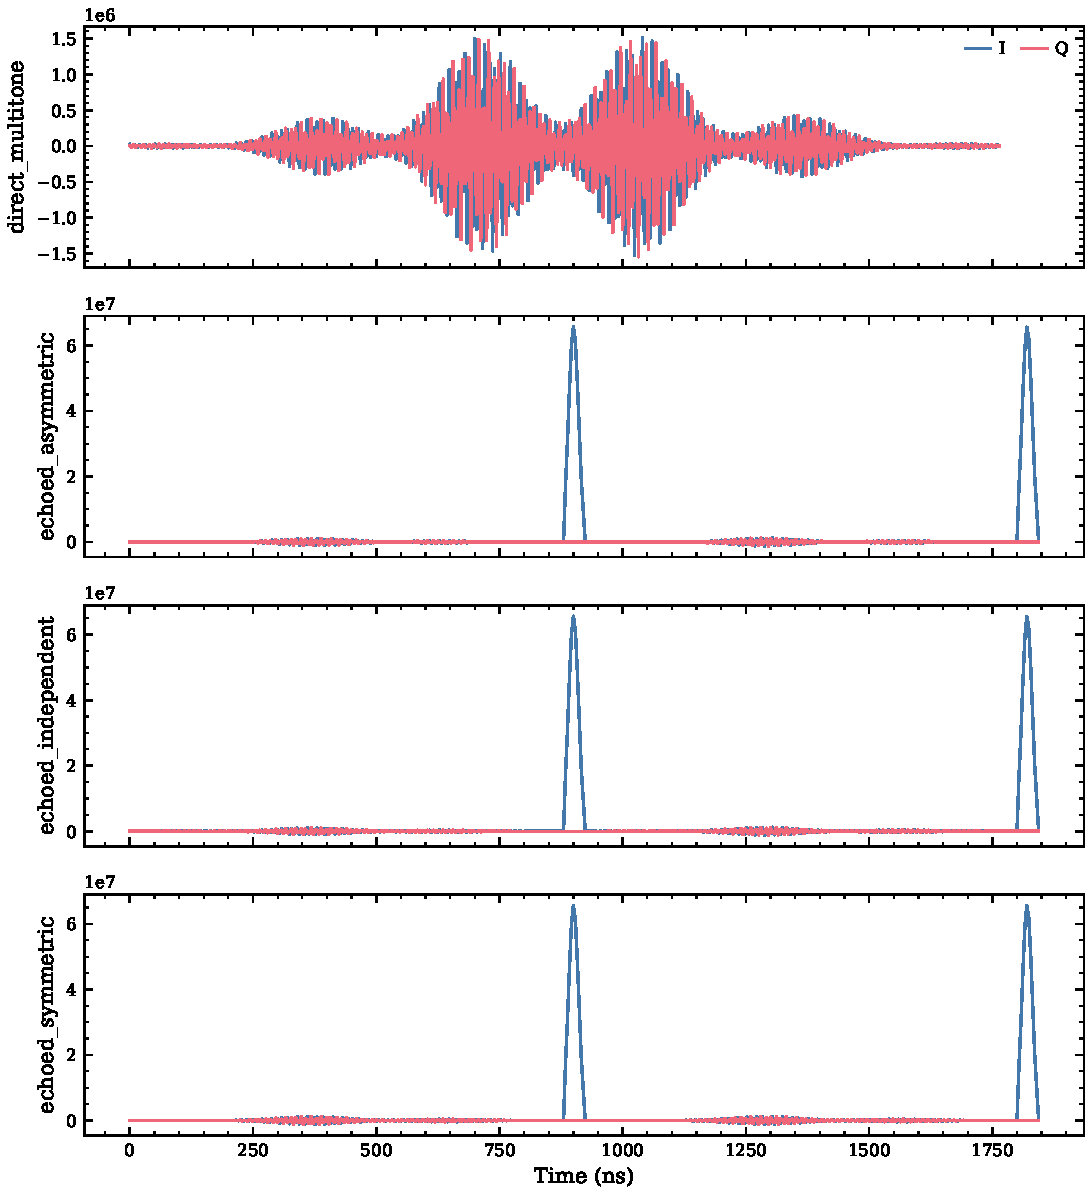
\includegraphics[width=\textwidth]{../figures/representative_waveforms.pdf}
\caption{Representative direct and echoed baseband waveforms for a difficult case. The echoed constructions split the active drive into two halves and add finite refocusing pulses, increasing total sequence length without improving the final gate quality.}
\label{fig:appendix_waveforms}
\end{figure*}

\section{Reproducibility}

\subsection{Optimized Parameters}
The best direct case uses two active tones. Its optimized corrections are
\begin{align}
\delta\lambda &= (0.02613,\,-0.00892),\\
\delta\alpha &= (0.04008,\;0.02582)\ \mathrm{rad},\\
\delta\omega/2\pi &= (-4.32\times 10^{-5},\;8.38\times 10^{-4})\ \mathrm{Hz}.
\end{align}
The corresponding tone amplitudes are $2.90979\times 10^5$ and $4.20303\times 10^5$ rad/s.

The best echoed case is the saved asymmetric artifact for \texttt{chi\_plus\_chiprime\_staggered\_x\_na2\_chiT3p0}, although its fitted asymmetry is $\eta=0$. Segment 1 corrections are
\begin{align}
\delta\lambda^{(1)} &= (0.13985,\;0.26531),\\
\delta\alpha^{(1)} &= (-0.02455,\;0.29819)\ \mathrm{rad},\\
\delta\omega^{(1)}/2\pi &= (-1.30\times 10^{-7},\;-1.5420\times 10^{-3})\ \mathrm{Hz},
\end{align}
and segment 2 corrections are
\begin{align}
\delta\lambda^{(2)} &= (0.11411,\;0.27894),\\
\delta\alpha^{(2)} &= (-0.01660,\;0.06620)\ \mathrm{rad},\\
\delta\omega^{(2)}/2\pi &= (-7.41\times 10^{-10},\;-1.5420\times 10^{-3})\ \mathrm{Hz}.
\end{align}

\subsection{Waveform and Pulse Information}
The direct waveform uses a single Gaussian-envelope multitone pulse of duration \SI{1760.56}{\nano\second} in the best case. The echoed constructions use two Gaussian half-SQR segments plus two Gaussian $X_\pi$ pulses of duration \SI{40}{\nano\second} each. In the best echoed case the two half segments are each \SI{528.17}{\nano\second}, so the total gate duration is \SI{1136.34}{\nano\second}.

Machine-readable waveform samples are stored in \texttt{artifacts/waveforms/*.npz}. Each file contains the sampled time array, the real and imaginary baseband waveform, and the distorted waveform arrays.

\subsection{Gate Sequence and Decomposition}
The direct construction is a single multitone qubit drive. The echoed construction is
\begin{enumerate}
  \item multitone half-SQR segment,
  \item finite Gaussian $X_\pi$ pulse,
  \item multitone half-SQR segment,
  \item finite Gaussian $X_\pi$ pulse.
\end{enumerate}
All pulses act on the qubit drive channel, and all simulations use the same qubit-first tensor ordering as the rest of the repository.

\subsection{Modeling and Simulation Assumptions}
The working Hilbert space uses a two-level qubit and a cavity truncation of $N_{\mathrm{active}}+2$ in the main runs. The solver uses the frame matched to $(\omega_q,\omega_c)$, the compiled time step is \SI{4}{\nano\second} in the main runs, and no decoherence channels are included. The study is therefore a closed-system unitary-control comparison, not a noisy hardware benchmark.

\subsection{Reproduction Procedure}
The study can be reproduced from the saved scripts and artifacts as follows.
\begin{enumerate}
  \item Run \texttt{python studies/ideal\_sqr\_direct\_vs\_echoed\_multitone/scripts/run\_study.py} to regenerate the 64 construction rows, figures, JSON summaries, CSV table, and machine-readable artifacts.
  \item Run \texttt{python studies/ideal\_sqr\_direct\_vs\_echoed\_multitone/scripts/validate\_results.py} to regenerate the sanity and convergence checks in \texttt{data/validation\_summary.json}.
  \item Open \texttt{scripts/reproducibility\_notebook.ipynb} for the saved-data walkthrough, or compile this report with \texttt{pdflatex}, \texttt{bibtex}, and \texttt{pdflatex} twice.
  \item Verify agreement by checking that the best direct case again reaches average fidelity near $0.72454$, the best echoed case near $0.31134$, and the figures match those stored in \texttt{figures/}.
\end{enumerate}

\subsection{Saved Artifacts}
The following machine-readable outputs are created by the study:
\begin{itemize}
  \item \texttt{data/study\_results.json}: complete list of the 64 construction rows.
  \item \texttt{data/study\_results.csv}: flat table version of the same results.
  \item \texttt{data/study\_summary.json}: best-case summaries, construction averages, and direct-versus-echo deltas.
  \item \texttt{data/analytic\_summary.json}: low-dimensional analytic statements and audit findings.
  \item \texttt{data/validation\_summary.json}: sanity and convergence checks.
  \item \texttt{artifacts/cases/*.json}: per-case artifacts containing optimized parameters, restricted operators, diagnostics, and waveform metadata.
  \item \texttt{artifacts/waveforms/*.npz}: compact sampled waveforms for each saved construction.
\end{itemize}
Each case artifact JSON includes a \texttt{load\_instructions} field and can be inspected programmatically without rerunning the optimizer.

\end{document}
